\documentclass{article}

%opening
\title{Simulating Different Receivers in a \\Rayleigh Fading, MIMO Environment\\
\large Project \#2}
\author{Intelligent Communication Systems (ICS) Lab.\\노용재}
\date{Winter Intern Seminar (2023-1)}

\usepackage{kotex} % korean
\usepackage[margin=1in]{geometry} % 둘레 margin
\usepackage{matlab-prettifier}
\usepackage{amsmath}
\usepackage{graphicx} % image
\usepackage{subcaption}
\usepackage{xcolor} % for coloring text
\usepackage{amssymb} % because, therefore symbol
\usepackage{float}
\usepackage{wrapfig}

\newcommand{\bd}{\textbf} % bold
\providecommand{\abs}[1]{\lvert#1\rvert}
\graphicspath{{./img/}}
\newcommand{\sgn}{\operatorname{sgn}}
\begin{document}

\maketitle
\tableofcontents
\vspace{0.5cm}
\hrule
\vspace{0.5cm}

\section{Implementation}
\begin{lstlisting}[style=Matlab-editor, frame=single, numbers=left,]
% Environment Variables
Nr = Nt
NormalizationFactor = sqrt(2/3*(M-1)*Nt);

% Signal Generation
SignalSequence = randi([0 M-1], Nt, 1);
SignalBinary = de2bi(SignalSequence, log2(M), 'left-msb');
SymbolSequence = qammod(SignalSequence, M) / NormalizationFactor;

% Noise (n) Generation
NoiseSequence = (randn(Nt, 1) + 1j * randn(Nt, 1)) / sqrt(2);
H = (randn(Nr, Nt) + 1j * randn(Nr, Nt)) ./ sqrt(2);
\end{lstlisting}
\textsl{Normalization Factor}를 $\sqrt{\frac{2}{3}(M-1)N_t}$로 설정한 이유는 하나의 trasmitter가 $\frac{1}{N_t}$W의 전력을 갖도록 하기 위해서이다.
\begin{figure}[H]
	\centerline{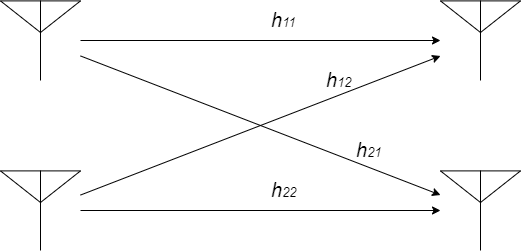
\includegraphics[width=0.5\textwidth]{antenna.png}}
	\caption{}
\end{figure}
\begin{gather}
	\begin{split}
		H &=
		\begin{bmatrix}
		h_{11} & \hdots & h_{1N_T}\\
		\vdots & \ddots & \vdots\\
		h_{N_R1} & \hdots & h_{N_R N_T}
		\end{bmatrix}
	\end{split}
\end{gather}
\subsection{ZF(Zero-forcing)}
\bd{Moore Penrose Pseudo Inverse}\\
$W_{ZF}H=I$를 만족하는 $W_{ZF}$를 찾으려고 한다. $H^H H$는 square matrix라는 사실을 이용하여 $W_{ZF}$를 구할 수 있다는 사실을 이용해 $W_{ZF}=(H^H H)^{-1}H^H$임을 알 수 있다.
\begin{gather}
	\begin{split}
		W_{ZF}H&=(H^H H)^{-1}H^H H\\
		&=(H^H H)^{-1}(H^H H) \quad (\because associative\ property)\\
		&=I
	\end{split}
\end{gather}
이때, $W_{ZF}$를 $H$의 \textsl{right pseudo-inverse}라고 할 수 있다.\\
\textsl{Matlab}에는 Moore Penrose Pseudo Inverse를 구할 수 있는 \bd{pinv(H)} 함수가 존재한다.
\begin{lstlisting}[style=Matlab-editor, frame=single, numbers=left,]
% ZF Receiver
w_zf = pinv(H); % pinv(H) = inv(H' * H) * H'
DetectedSymbolSequence_ZF = w_zf * ReceivedSymbolSequence;

% Detection
DetectedSignalSequence_ZF = qamdemod(DetectedSymbolSequence_ZF*NormalizationFactor, M);
DetectedBinary_ZF = de2bi(DetectedSignalSequence_ZF, log2(M), 'left-msb');

BitErrorCount_ZF(indx_EbN0) = BitErrorCount_ZF(indx_EbN0) + sum(SignalBinary~=DetectedBinary_ZF, 'all');
SignalErrorCount_ZF(indx_EbN0) = SignalErrorCount_ZF(indx_EbN0) + sum(SignalSequence~=DetectedSignalSequence_ZF, 'all');
\end{lstlisting}
\subsection{MMSE(Minimum Mean Square Error)}
\begin{gather}
	W_{MMSE}=\sqrt{\frac{N_t}{E_s}}(H^H+\frac{N_t}{\rho})^{-1}H^H
\end{gather}
\begin{lstlisting}[style=Matlab-editor, frame=single, numbers=left,]
% MMSE Receiver
w_mmse = inv(H' * H + Nt / EsN0(indx_EbN0) * eye(Nr)) * H';
DetectedSymbolSequence_MMSE = w_mmse * ReceivedSymbolSequence; % Detection (Zero-Forcing: y / h)

DetectedSignalSequence_MMSE = qamdemod(DetectedSymbolSequence_MMSE*NormalizationFactor, M); % Detection
DetectedBinary_ZF = de2bi(DetectedSignalSequence_MMSE, log2(M), 'left-msb');

BitErrorCount_MMSE(indx_EbN0) = BitErrorCount_MMSE(indx_EbN0) + sum(SignalBinary~=DetectedBinary_ZF, 'all');
SignalErrorCount_MMSE(indx_EbN0) = SignalErrorCount_MMSE(indx_EbN0) + sum(SignalSequence~=DetectedSignalSequence_MMSE, 'all');
\end{lstlisting}
\subsection{MLD(Maximum Likelihood Detection)}
\bd{Creating All Possible Signal Combinations}
\begin{lstlisting}[style=Matlab-editor, frame=single, numbers=left,]
% Creating Matrix for all possible combinations of signals (M^Nt possible combinations)
AllNumbers = de2bi([0:M^Nt-1], Nt*log2(M), 'left-msb');
Candidates = zeros(M^Nt, Nt);
for ii = 1 : M^Nt
    for jj = 1 : Nt
        Candidates(ii,jj) = bi2de(AllNumbers(ii,log2(M)*(jj-1)+1:log2(M)*jj), 'left-msb');
    end
end
Candidates = qammod(Candidates',M) / NormalizationFactor;
\end{lstlisting}
\textsl{AllNumbers}는 각 열마다 0부터 $M^{N_t}-1$를 이진수로 나태낸 matrix이다.
\begin{figure}[H]
	\centerline{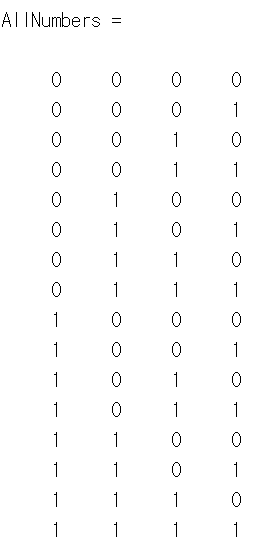
\includegraphics[width=0.2\textwidth]{AllNumbers.png}}
	\caption{$M=4$, $N_t=2$}
\end{figure}
\bd{Figure 2}은 $M=4$, $N_t=2$일 때의 \textsl{AllNumbers}의 예시이다. \textsl{AllNumbers}의 각 열을 $\log_{2}M$ 숫자의 묶음이 $N_t$개로 있는 것으로 생각한다. 그렇다면, 각 열은 가능한 하나의 signal combination으로 볼 수 있다. \textsl{Candidates}의 dimension은 $M^{N_t}\times N_t$이다. 이는 $N_t$개의 signal로 만들 수 있는 $M^{N_t}$개의 signal combination을 나타낸다.\\
\\
\bd{Solving For Minimum Euclidean Distance}
\begin{gather}
\hat{s}=\operatorname*{argmin}_s \abs{y-Hs}^2
\end{gather}
\begin{lstlisting}[style=Matlab-editor, frame=single, numbers=left,]
% MLD Receiver
% 'EulcideanDistance' results in Nt x M^Nt, each column representing each candidate symbol combination
EuclideanDistance = abs(ReceivedSymbolSequence * ones(1,M^Nt) - H*Candidates).^2;
[val, idx] = min(sum(EuclideanDistance, 1));
DetectedBinary_MLD = reshape(de2bi(idx-1, log2(M)*Nt, 'left-msb'),log2(M),[])';
DetectedSequence_MLD = bi2de(DetectedBinary_MLD, 'left-msb');

BitErrorCount_MLD(indx_EbN0) = BitErrorCount_MLD(indx_EbN0) + sum(SignalBinary~=DetectedBinary_MLD, 'all');
SignalErrorCount_MLD(indx_EbN0) = SignalErrorCount_MLD(indx_EbN0) + sum(SignalSequence~=DetectedSequence_MLD, 'all');
\end{lstlisting}
\begin{gather}
ReceivedSymbolSequence=[y_1\ \hdots\ y_{N_R}]^T
\end{gather}
\textsl{sum(EuclideanDistance, 1)}는 $\Vert y-Hs\Vert_F^2$을 의미한다.
\section{결과 및 분석}
\subsection{Simulation Result}
\begin{figure}[H]
	\centering
	\begin{subfigure}{0.5\textwidth}
		\centerline{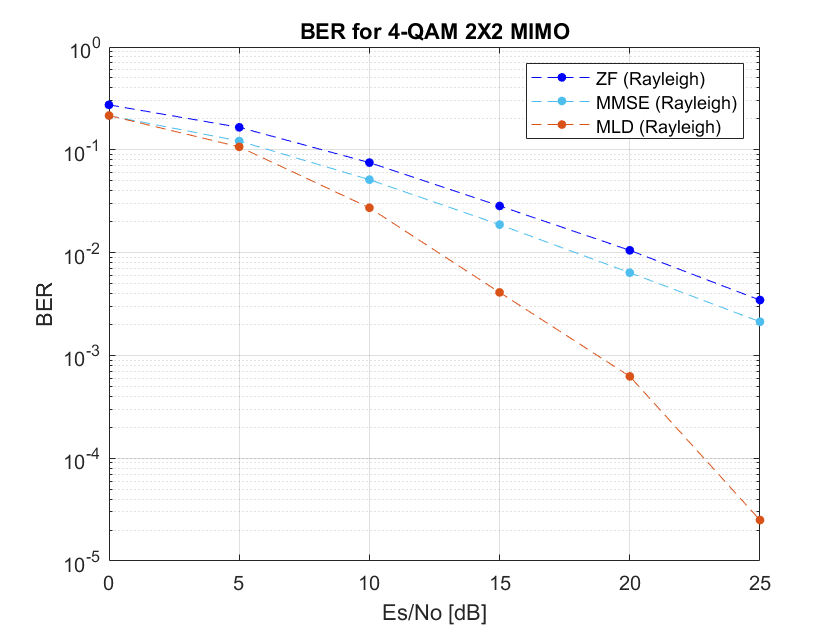
\includegraphics[width=1\textwidth]{a_Es_BER.png}}
		\caption{BER}
	\end{subfigure}%
	\begin{subfigure}{0.5\textwidth}
		\centerline{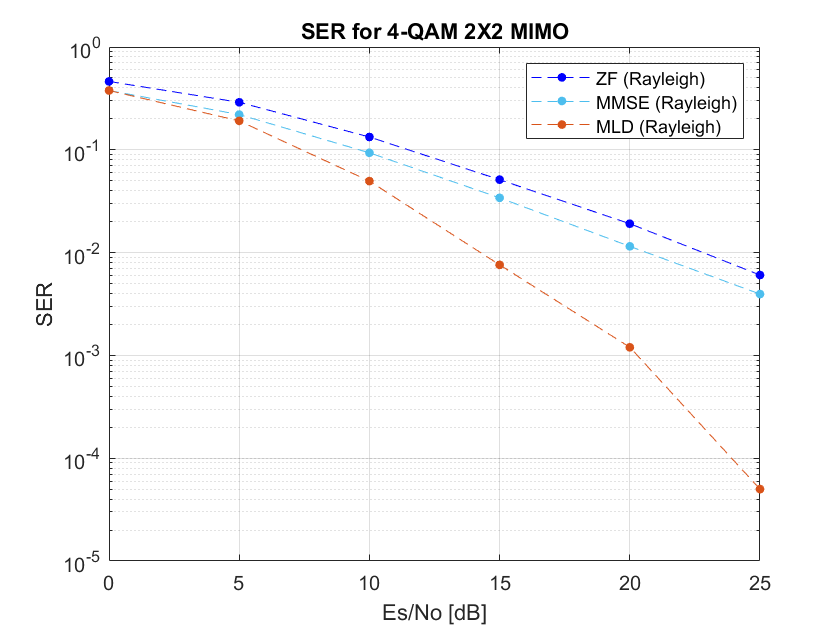
\includegraphics[width=1\textwidth]{a_Es_SER.png}}
		\caption{SER}
	\end{subfigure}\\%
	\begin{subfigure}{0.5\textwidth}
		\centerline{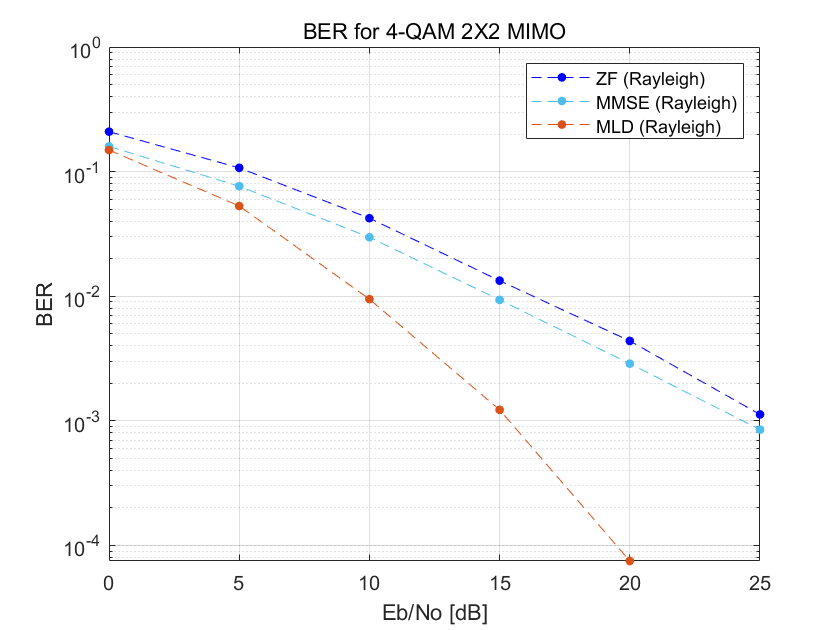
\includegraphics[width=1\textwidth]{a_Eb_BER.png}}
		\caption{BER}
	\end{subfigure}%
	\begin{subfigure}{0.5\textwidth}
		\centerline{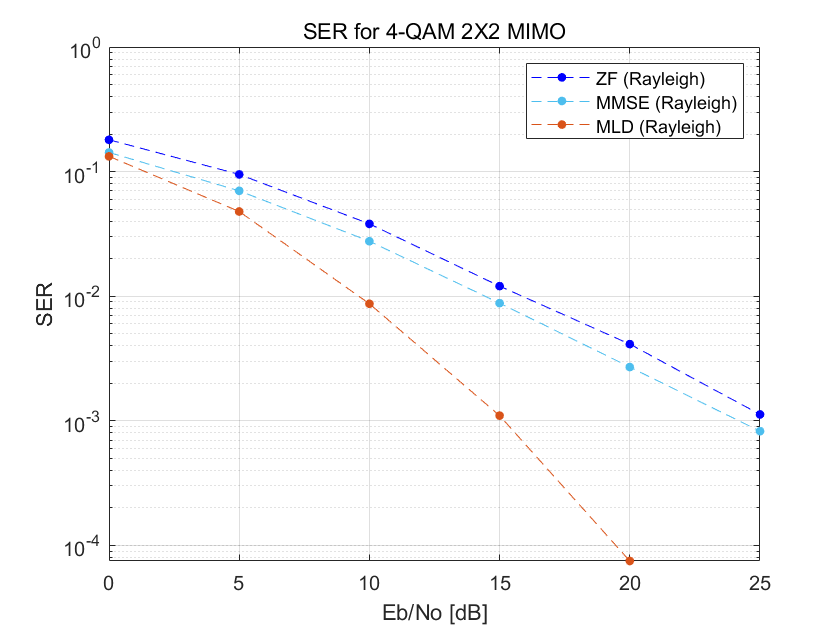
\includegraphics[width=1\textwidth]{a_Eb_SER.png}}
		\caption{SER}
	\end{subfigure}%
	\caption{4-QAM 2$\times$2 MIMO}
\end{figure}
\begin{figure}[H]
	\centering
	\begin{subfigure}{0.5\textwidth}
		\centerline{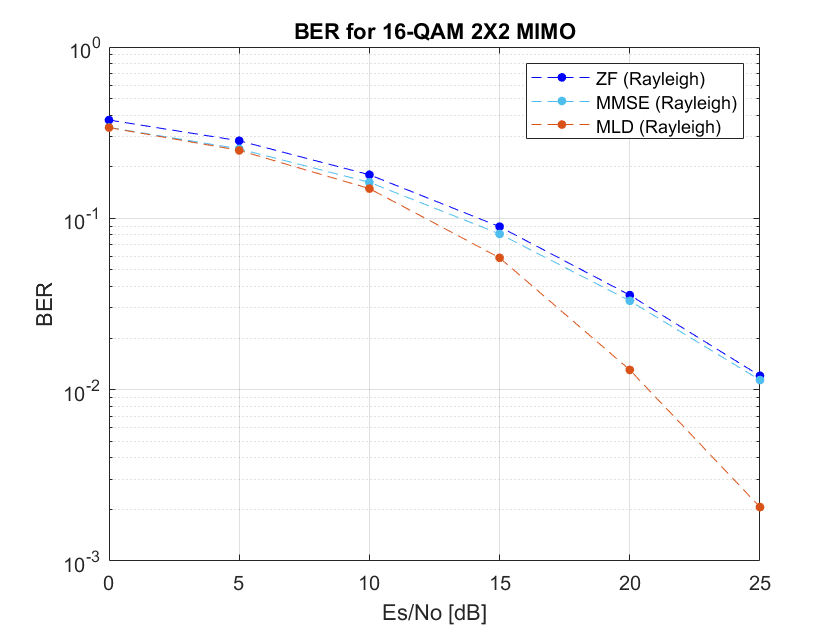
\includegraphics[width=1\textwidth]{b_Es_BER.png}}
		\caption{BER}
	\end{subfigure}%
	\begin{subfigure}{0.5\textwidth}
		\centerline{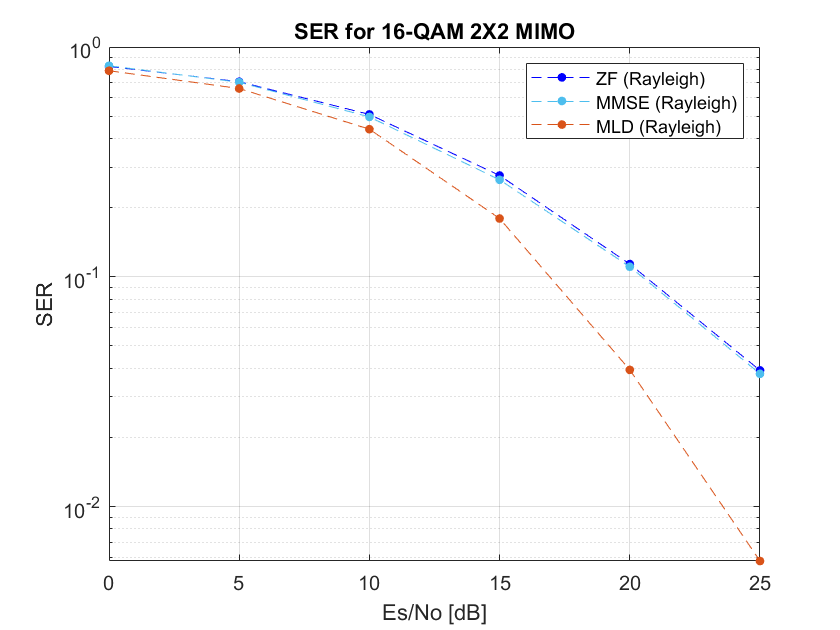
\includegraphics[width=1\textwidth]{b_Es_SER.png}}
		\caption{SER}
	\end{subfigure}\\%
	\begin{subfigure}{0.5\textwidth}
		\centerline{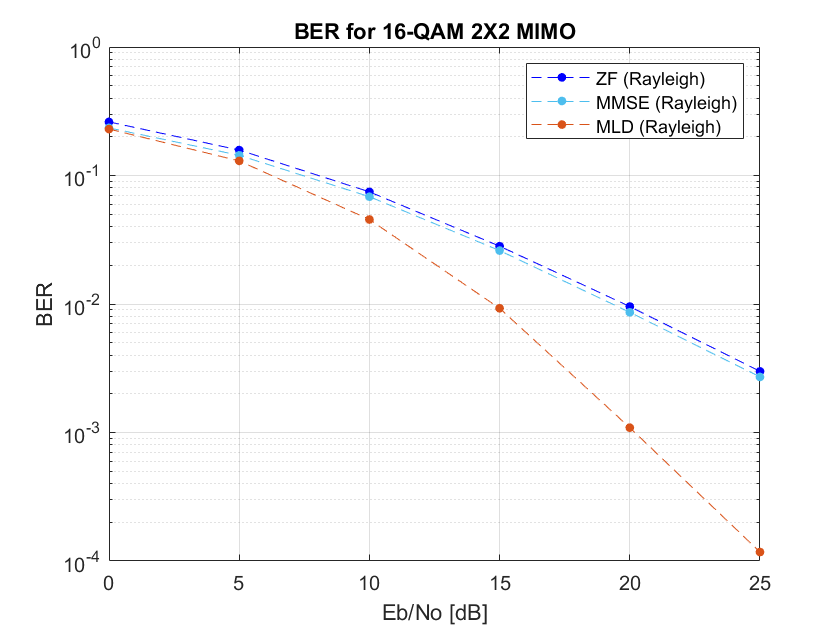
\includegraphics[width=1\textwidth]{b_Eb_BER.png}}
		\caption{BER}
	\end{subfigure}%
	\begin{subfigure}{0.5\textwidth}
		\centerline{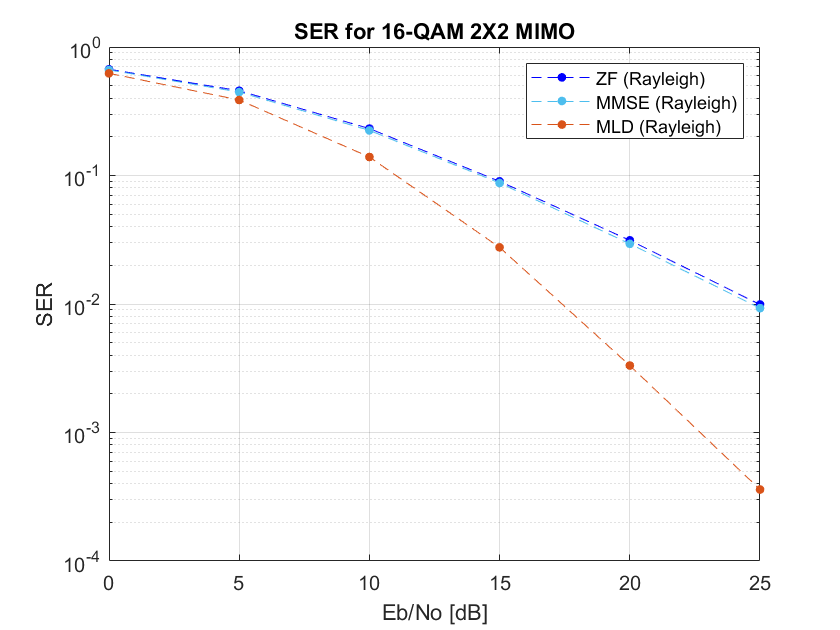
\includegraphics[width=1\textwidth]{b_Eb_SER.png}}
		\caption{SER}
	\end{subfigure}%
	\caption{16-QAM 2$\times$2 MIMO}
\end{figure}
\begin{figure}[H]
	\centering
	\begin{subfigure}{0.5\textwidth}
		\centerline{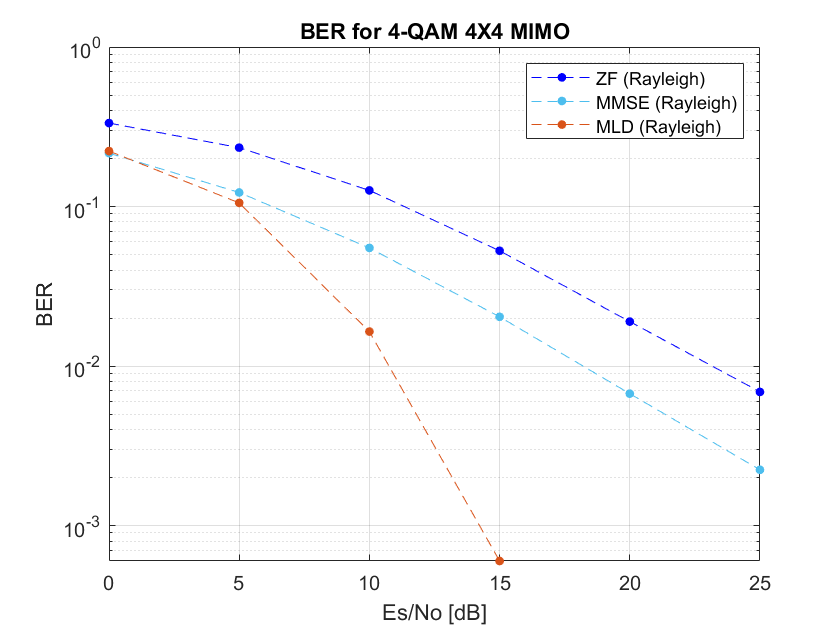
\includegraphics[width=1\textwidth]{c_Es_BER.png}}
		\caption{BER}
	\end{subfigure}%
	\begin{subfigure}{0.5\textwidth}
		\centerline{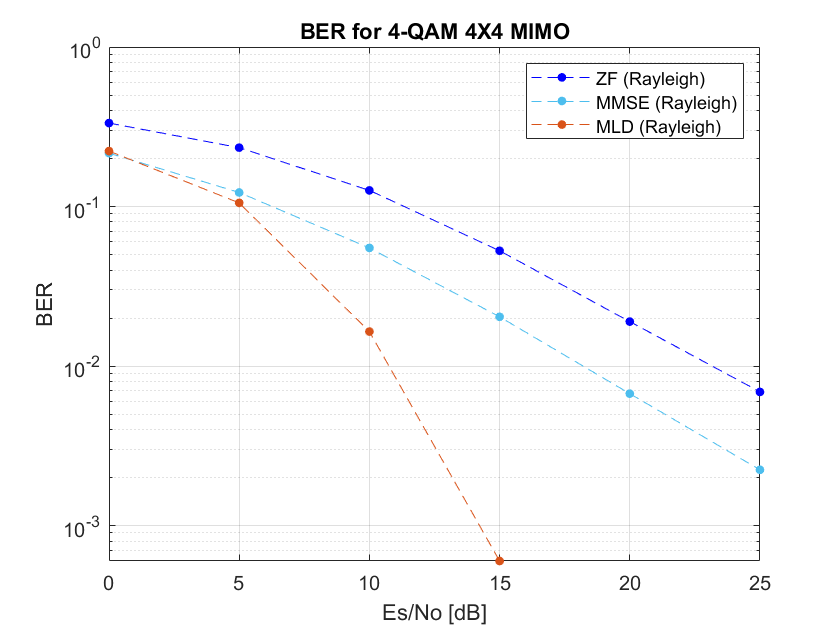
\includegraphics[width=1\textwidth]{c_Es_BER.png}}
		\caption{SER}
	\end{subfigure}\\%
	\begin{subfigure}{0.5\textwidth}
		\centerline{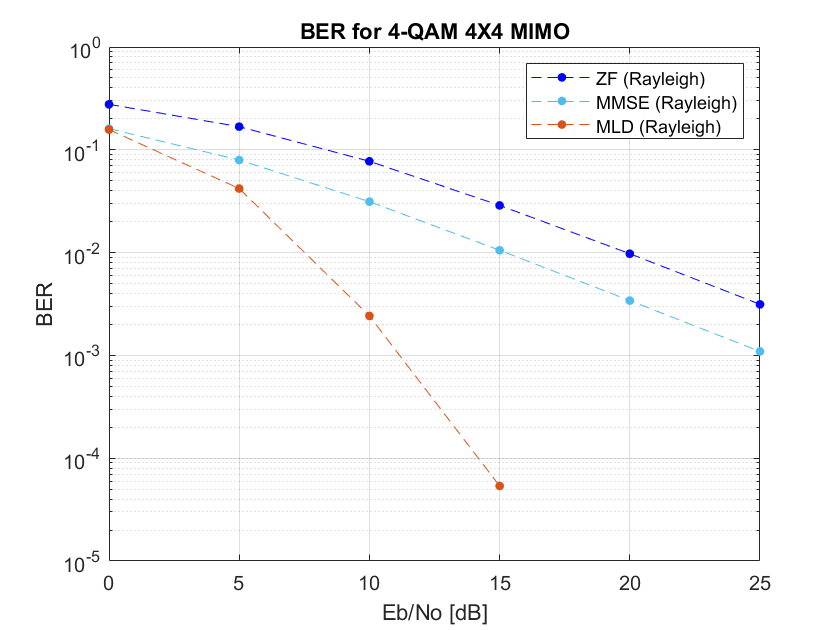
\includegraphics[width=1\textwidth]{c_Eb_BER.png}}
		\caption{BER}
	\end{subfigure}%
	\begin{subfigure}{0.5\textwidth}
		\centerline{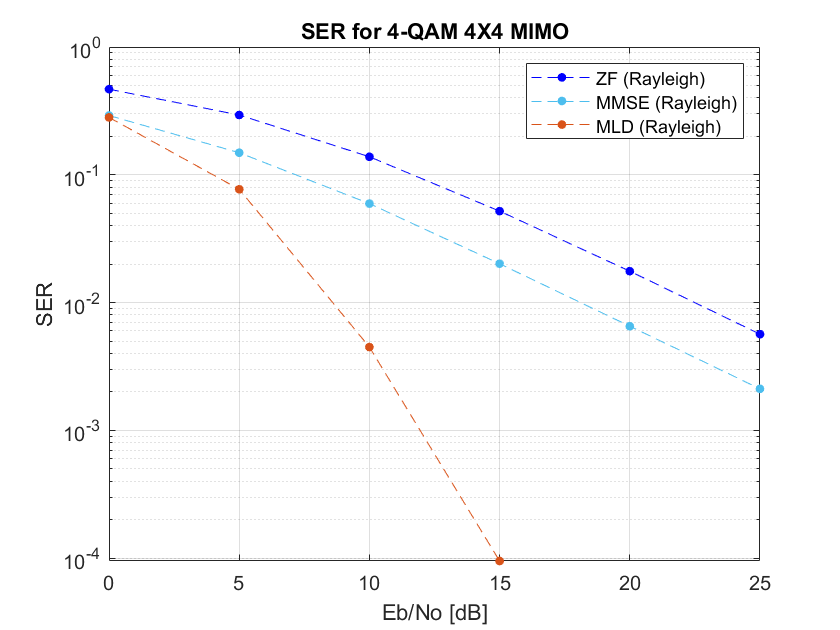
\includegraphics[width=1\textwidth]{c_Eb_SER.png}}
		\caption{SER}
	\end{subfigure}%
	\caption{4-QAM 4$\times$4 MIMO}
\end{figure}
\begin{figure}[H]
	\centering
	\begin{subfigure}{0.5\textwidth}
		\centerline{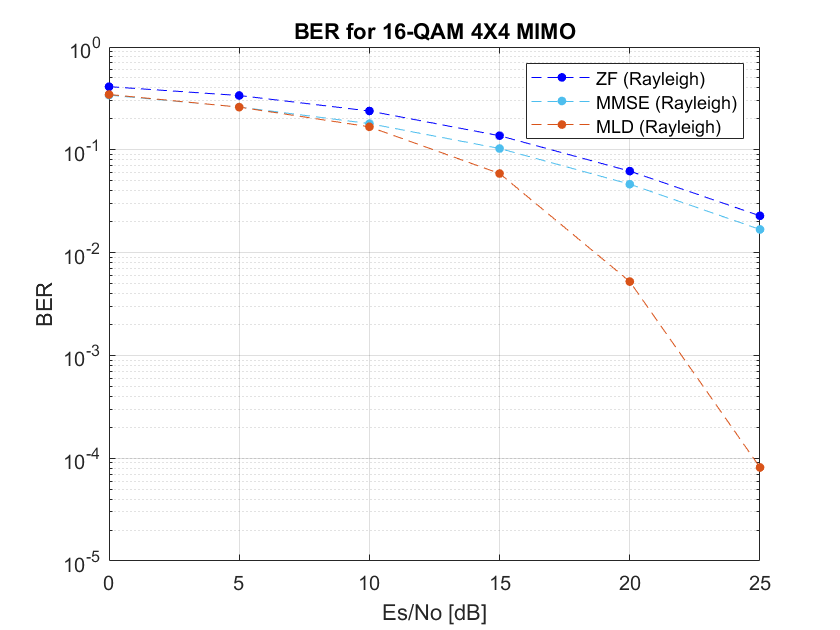
\includegraphics[width=1\textwidth]{d_Es_BER.png}}
		\caption{BER}
	\end{subfigure}%
	\begin{subfigure}{0.5\textwidth}
		\centerline{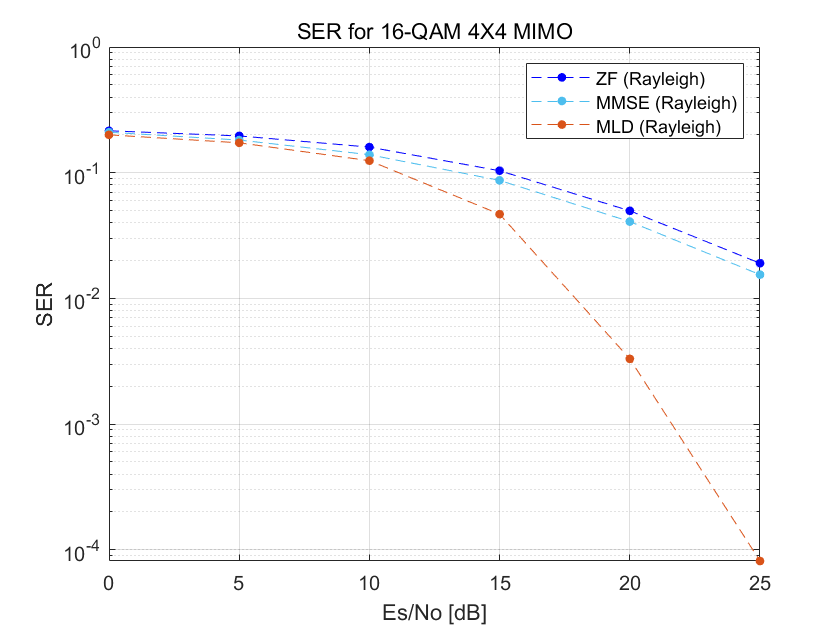
\includegraphics[width=1\textwidth]{d_Es_SER.png}}
		\caption{SER}
	\end{subfigure}\\%
	\begin{subfigure}{0.5\textwidth}
		\centerline{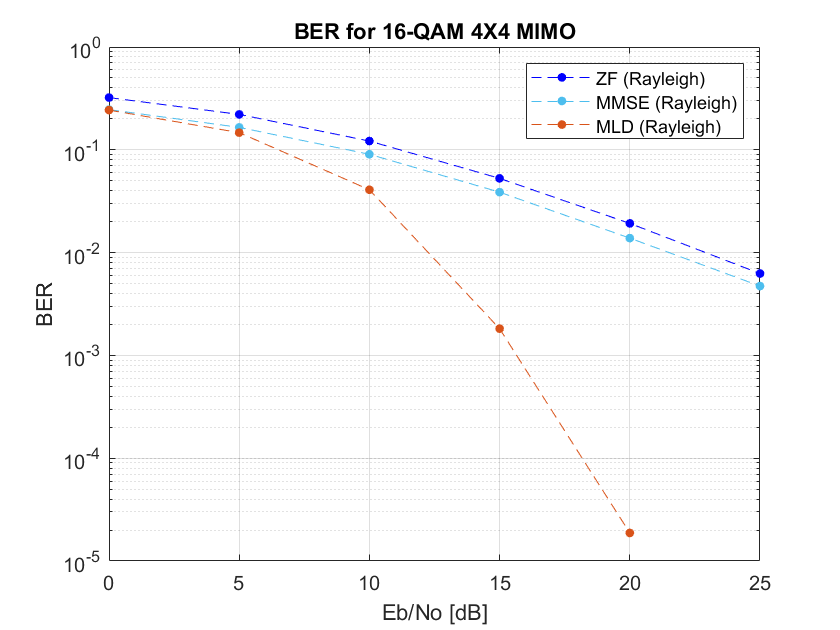
\includegraphics[width=1\textwidth]{d_Eb_BER.png}}
		\caption{BER}
	\end{subfigure}%
	\begin{subfigure}{0.5\textwidth}
		\centerline{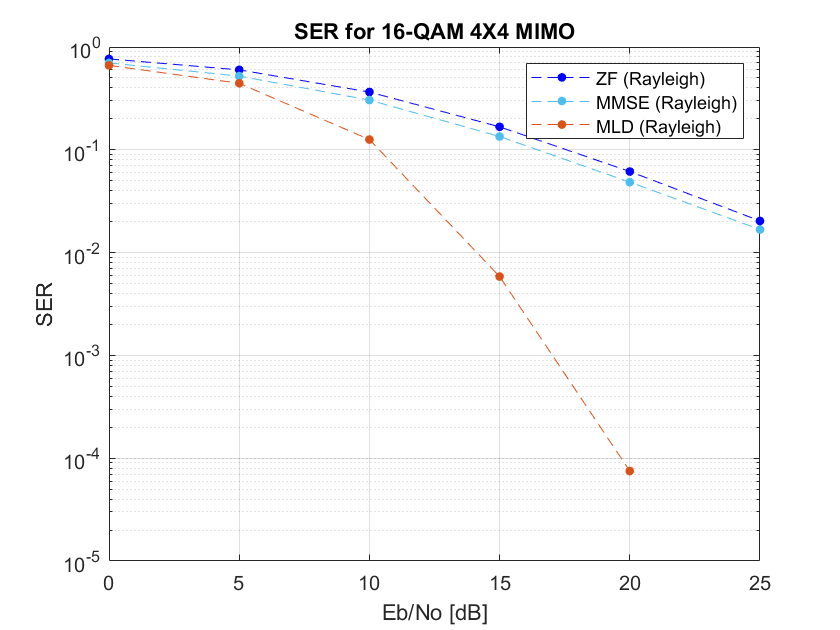
\includegraphics[width=1\textwidth]{d_Eb_SER.png}}
		\caption{SER}
	\end{subfigure}%
	\caption{16-QAM 4$\times$4 MIMO}
\end{figure}
\section{미해결 \& 추가연구 필요 내용}
\begin{itemize}
  \item $W_{ZF}=(H^H H)^{-1}H^H$, transpose를 한다고 하더라도 동일한 결과를 가져오는 것 아닌가? 왜 ZF에서 transpose가 아닌 hermitian transpose를 사용한건가?
\end{itemize}
\section[Entire Code]{Entire Code \footnote{Uploaded on https://github.com/lightwick/ICS\textunderscore project/blob/main/MIMO\textunderscore Rayleigh/main.m}}
\begin{lstlisting}[style=Matlab-editor, frame=single, numbers=left,]
close all
clear
clc

Es = 1;

% Environment Varible
M = 16
Nt = 2
Nr = Nt
NumberIteration = 10^5;
NumberOfSignals = 1;

% Simulation
LengthBitSequence = Nt * log2(M); % log2(M) bits per signal
NormalizationFactor = sqrt(2/3*(M-1)*Nt);

EbN0_dB = 0:5:25;
EbN0 = db2pow(EbN0_dB);

EsN0 = EbN0 * log2(M);
EsN0_db = pow2db(EsN0);

BitErrorCount_ZF = zeros(1, length(EsN0_db));
SignalErrorCount_ZF = zeros(1, length(EsN0_db));

BitErrorCount_MLD = zeros(1, length(EsN0_db));
SignalErrorCount_MLD = zeros(1, length(EsN0_db));

BitErrorCount_MMSE = zeros(1, length(EsN0_db));
SignalErrorCount_MMSE = zeros(1, length(EsN0_db));

AllNumbers = de2bi([0:M^Nt-1], Nt*log2(M), 'left-msb');
Candidates = zeros(M^Nt, Nt);
for ii = 1 : M^Nt
    for jj = 1 : Nt
        Candidates(ii,jj) = bi2de(AllNumbers(ii,log2(M)*(jj-1)+1:log2(M)*jj), 'left-msb');
    end
end
Candidates = qammod(Candidates',M) / NormalizationFactor;

for iTotal = 1 : NumberIteration
    if mod(iTotal-1, FivePercent)==0
        tic
    end
    % Bit Generation
    SignalSequence = randi([0 M-1], Nt, 1);
    SignalBinary = de2bi(SignalSequence, log2(M), 'left-msb');
    SymbolSequence = qammod(SignalSequence, M) / NormalizationFactor;
    
    NoiseSequence = (randn(Nt, 1) + 1j * randn(Nt, 1)) / sqrt(2); % Noise (n) Generation
    H = (randn(Nr, Nt) + 1j * randn(Nr, Nt)) ./ sqrt(2); % Receiver x Transmitter
    for indx_EbN0 = 1 : length(EsN0)
        % Received Signal (y = hs + n) Generation
        ReceivedSymbolSequence = H * SymbolSequence + NoiseSequence * sqrt(1 / EsN0(indx_EbN0)); % log2(M)x1 matrix
        
        % MLD Receiver
        EuclideanDistance = abs(ReceivedSymbolSequence * ones(1,M^Nt) - H*Candidates).^2; % results in Nt x M^Nt, each column representing each candidate symbol combination
        [val, idx] = min(sum(EuclideanDistance, 1));
        DetectedBinary_MLD = reshape(de2bi(idx-1, log2(M)*Nt, 'left-msb'),log2(M),[])'; % MOST LIKELY WRONG
        DetectedSequence_MLD = bi2de(DetectedBinary_MLD, 'left-msb');
        
        BitErrorCount_MLD(indx_EbN0) = BitErrorCount_MLD(indx_EbN0) + sum(SignalBinary~=DetectedBinary_MLD, 'all');
        SignalErrorCount_MLD(indx_EbN0) = SignalErrorCount_MLD(indx_EbN0) + sum(SignalSequence~=DetectedSequence_MLD, 'all');
        
        % ZF Receiver
        w_zf = pinv(H); % pinv(H) = inv(H' * H) * H'
        DetectedSymbolSequence_ZF = w_zf * ReceivedSymbolSequence; % Detection (Zero-Forcing: y / h)
        
        DetectedSignalSequence_ZF = qamdemod(DetectedSymbolSequence_ZF*NormalizationFactor, M); % Detection
        DetectedBinary_ZF = de2bi(DetectedSignalSequence_ZF, log2(M), 'left-msb');
        
        BitErrorCount_ZF(indx_EbN0) = BitErrorCount_ZF(indx_EbN0) + sum(SignalBinary~=DetectedBinary_ZF, 'all');
        SignalErrorCount_ZF(indx_EbN0) = SignalErrorCount_ZF(indx_EbN0) + sum(SignalSequence~=DetectedSignalSequence_ZF, 'all');
        
        % MMSE Receiver
        w_mmse = inv(H' * H + Nt / EsN0(indx_EbN0) * eye(Nr)) * H';
        DetectedSymbolSequence_MMSE = w_mmse * ReceivedSymbolSequence; % Detection (Zero-Forcing: y / h)
        
        DetectedSignalSequence_MMSE = qamdemod(DetectedSymbolSequence_MMSE*NormalizationFactor, M); % Detection
        DetectedBinary_ZF = de2bi(DetectedSignalSequence_MMSE, log2(M), 'left-msb');
        
        BitErrorCount_MMSE(indx_EbN0) = BitErrorCount_MMSE(indx_EbN0) + sum(SignalBinary~=DetectedBinary_ZF, 'all');
        SignalErrorCount_MMSE(indx_EbN0) = SignalErrorCount_MMSE(indx_EbN0) + sum(SignalSequence~=DetectedSignalSequence_MMSE, 'all');
    end
end

SER_MLD = SignalErrorCount_MLD / (LengthBitSequence * NumberIteration);
BER_MLD = BitErrorCount_MLD / (LengthBitSequence * NumberIteration);

SER_ZF = SignalErrorCount_ZF / (LengthBitSequence * NumberIteration);
BER_ZF = BitErrorCount_ZF / (LengthBitSequence * NumberIteration);

SER_MMSE = SignalErrorCount_MMSE / (LengthBitSequence * NumberIteration);
BER_MMSE = BitErrorCount_MMSE / (LengthBitSequence * NumberIteration);

% Plot
figure()

semilogy(EbN0_dB, BER_ZF, 'b.--', 'MarkerSize', 15);
hold on
semilogy(EbN0_dB, BER_MMSE, '.--', 'Color', "#4DBEEE", 'MarkerSize', 15);
semilogy(EbN0_dB, BER_MLD, '.--','Color', '#D95319', 'MarkerSize', 15);
ylabel('BER');
title(sprintf("BER for %d-QAM %dX%d MIMO", M, Nr, Nt));
grid on
legend('ZF (Rayleigh)', 'MMSE (Rayleigh)', 'MLD (Rayleigh)');
xlabel('Eb/No [dB]');

figure()
semilogy(EbN0_dB, SER_ZF, 'b.--', 'MarkerSize', 15);
hold on
semilogy(EbN0_dB, SER_MMSE, '.--', 'Color', "#4DBEEE", 'MarkerSize', 15); 
semilogy(EbN0_dB, SER_MLD, '.--', 'Color', '#D95319', 'MarkerSize', 15);
ylabel('SER');
title(sprintf("SER for %d-QAM %dX%d MIMO", M, Nr, Nt));
grid on
legend('ZF (Rayleigh)', 'MMSE (Rayleigh)', 'MLD (Rayleigh)');
xlabel('Eb/No [dB]');
\end{lstlisting}
\end{document}